\subsection{4. Регулярные выражения. Теорема Клини о совпадении классов регулярных и автоматных языков. Регулярный автомат, алгоритм построения.}

\Vars \\
Regex (регулярное выражение) обозначим за $R$, \newline Language (язык) -- за $L$, \newline $L(R_i)$ (язык, который задается регулярным выражением $R$) -- $L_i$.

\Def Рекурсивное определение регулярного выражения.

% \begin{minipage}[r]{0.1\linewidth} 
% %\begin{flushright}
%     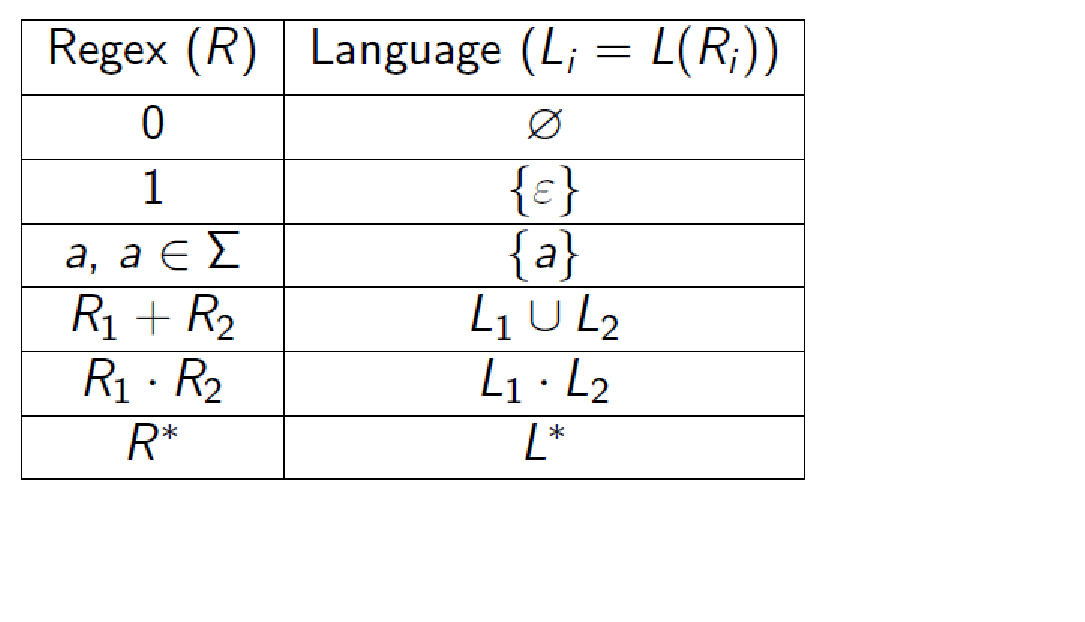
\includegraphics[width=5\linewidth]{images/1_4_1.png}
% %\end{flushright} 
% \end{minipage} 
\begin{center}
    \begin{tabular}{|c|c|}
        \hline
        $Regex (R)$ & $Language (L_i = L(R_i))$ \\
        \hline
        $0$ & $\varnothing$ \\
        $1$ & $\{ \varepsilon \}$ \\
        $a$, $a \in \Sigma$ & $\{ a \}$ \\
        $R_1 + R_2$ & $L_1 \cup L_2$ \\
        $R_1 \cdot R_2$ & $L_1 \cdot L_2$ \\
        $R^*$ & $L^*$ \\
        \hline
    \end{tabular}
\end{center}

Здесь $\varepsilon$ -- пустое слово, <<$\cdot$>> -- операция конкатенации языков (в полученном языке $L_1 \cdot L_2$ лежат слова вида $a_1a_2$, где слово $a_1$ лежит в языке $L_1$, а слово $a_2$ лежит в языке $L_2$), <<$*$>> -- звезда Клини.

Напомним определение звезды Клини: $V^* = \bigcup_{i=0}^{\infty} V^i$ 

\textbf{Приоритет операций} в регулярных выражениях (левее — приоритетнее): $* \rightarrow \cdot \rightarrow +$

\Def Язык $L$ -- регулярный, если он задается регулярным выражением.

\hspace{4ex}

\textbf{Теорема Клини:} Классы регулярных и автоматных языков совпадают.

\Proof Докажем два вложения:

\textbf{1. Регулярные $\subseteq$ Автоматные}

% \begin{figure}[h]
%     \begin{minipage}[h]{0.6\linewidth}
%     Индукция по построению выражения. 
    
%     Немного изменим утверждение -- докажем, что по регулярному выражению можно построить НКА с $1$ завершающим состоянием, который задает тот же язык.\\
    
%     \textit{База}: Построим автоматы для регулярных выражений: 0, 1, a.
%     \end{minipage}
%     \hspace{-4ex} \begin{minipage}[h]{0.5\linewidth}
%     \center{\includegraphics[width=0.6\linewidth]{images/4_base.jpg}}
%     \end{minipage}
% \end{figure}
% Регулярное выражение <<$0$>> -- автомат без завершающих состояний.

% Регулярное выражение <<$1$>> -- в автомате, состоящем из одной вершины, стартовая вершина помечается завершающим состоянием.

% Регулярное выражение <<$a$>> -- в автомате две вершины. Вершина номер $0$ стартовая, вершину номер $1$ помечаем как терминальную. Проводим ребро из $0$ в $1$, на котором пишем букву a.

Индукция по построению выражения. Немного изменим утверждение -- докажем, что по регулярному выражению можно построить НКА с $1$ завершающим состоянием, который задает тот же язык.

\textit{База}: Построим автоматы для регулярных выражений: $0, 1, a \in \Sigma$.
% %картинка%
\begin{figure}[h!]
    \centering
    \includegraphics[scale=0.27]{4_base.jpg}
\end{figure}
% \newline \center{\includegraphics[width=0.29\linewidth]{4_base.jpg}}
% \begin{minipage}[r]{1\linewidth} 
% %\begin{flushright}
%     % 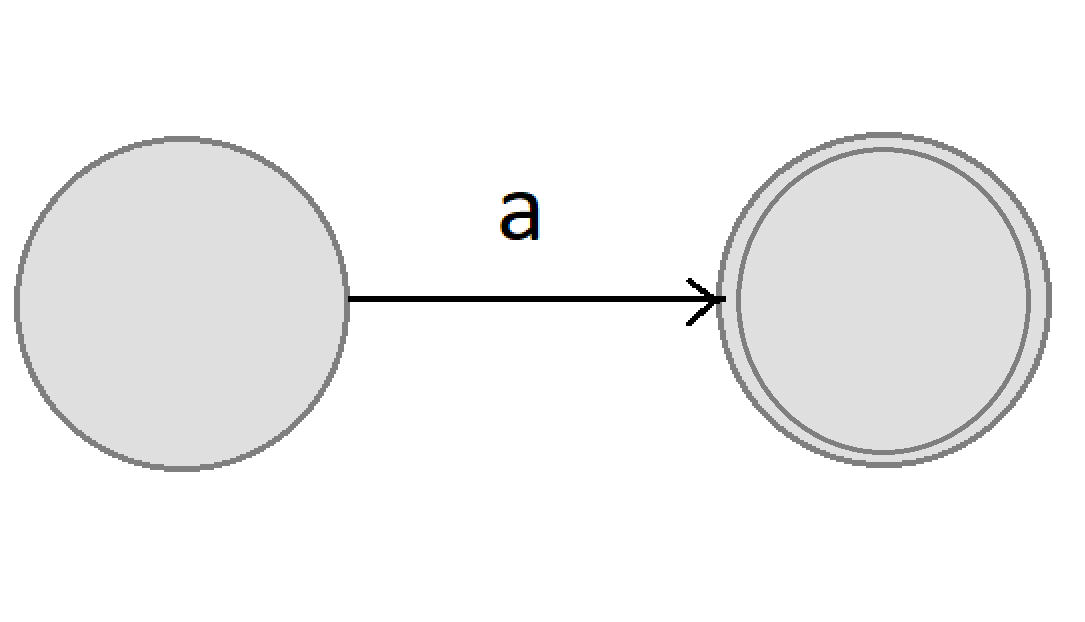
\includegraphics[width=2\linewidth]{images/1_4_2.png}
%     \center{\includegraphics[width=1\linewidth]{images/4_base.jpg}}
% %\end{flushright} 
% \end{minipage} 

\textit{Переход:}

1) $R = R_1 + R_2$. Построим автомат $A_1$ для $R_1$, для которого вершина $S_1$ -- стартовая, а вершина $F_1$ -- единственная терминальная. Для $R_2$ это будут автомат $A_2$ со стартовой вершиной $S_2$ и терминальной $F_2$.
Создадим новую вершину $S$, которая и будет стартовой в новом автомате. Из нее проведем два ребра с $\varepsilon$-переходами в $S_1$ и в $S_2$. Аналогично соединим завершающие в автоматах с новой завершающей вершиной $F$. Нетрудно доказать, что такой автомат задаст тот же язык, что и наше регулярное выражение.

2) $R = R_1 \cdot R_2$. Аналогично прошлому пункту получим автоматы для $R_1$ и $R_2$ с теми же обозначениями. Вершина $S_1$ будет стартовой в нашем новом автомате. Добавим также $\varepsilon$-переход из $F_1$ в $S_2$, уберем терминальность $F_1$.

3) $R = R_1^*$. Построим автомат $A_1$ для $R_1$ со стартовой вершиной $S_1$ и терминальной вершиной $F_1$. Создадим вершину $S$ -- новую стартовую вершину, пометим ее терминальной. Добавим из нее и из $F_1$ $\varepsilon$-переход в $S_1$.

\textbf{2. Автоматные $\subseteq$ Регулярные}

\Note{Регулярный автомат -- НКА, в котором на ребрах записаны регулярные выражения. Докажем утверждение для регулярных автоматов.}

\Note{Всякий НКА задается регулярным автоматом с 1 завершающим состоянием.}

Индукция по $|Q|$ (количеству состояний -- вершин) в регулярном автомате.

\textit{База:}

1) $|Q| = 1$. Тогда в регулярном автомате стартовое состояние является завершающим, и можно однозначно построить регулярное выражение. Такому автомату соответсвует регулярное выражение $a^*$
\newline
\begin{minipage}[r]{0.1\linewidth} 
%\begin{flushright}
    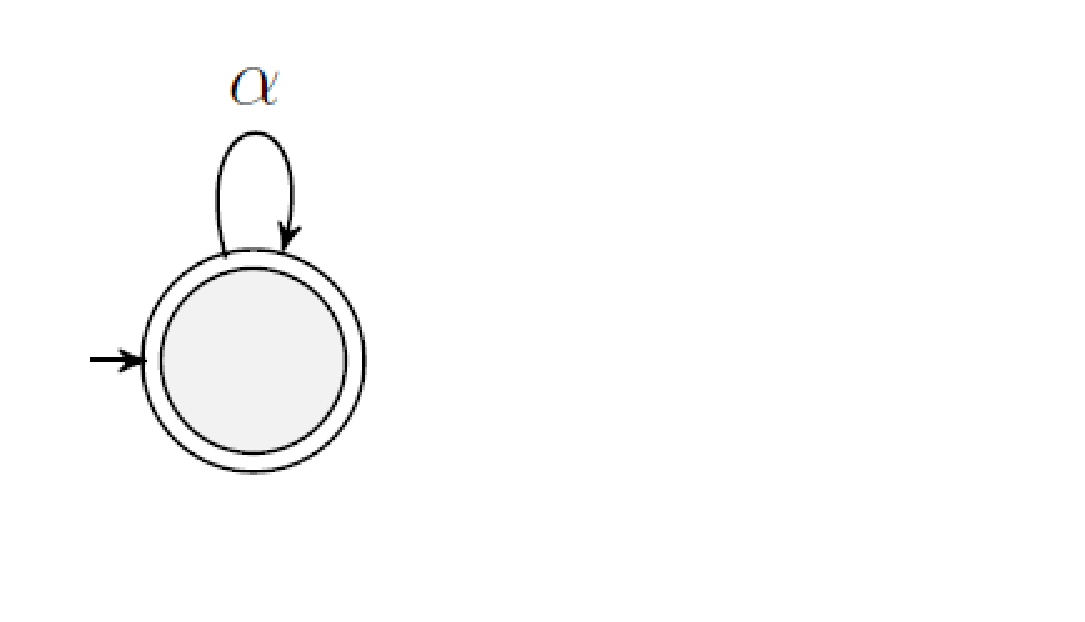
\includegraphics[width=4\linewidth]{images/1_4_3.png}
%\end{flushright} 
\end{minipage} 

2) $|Q| = 2$. Cтартовое состояние и завершающее состояние различны, и можно тоже однозначно построить регулярное выражение. Такому автомату соответсвует регулярное выражение $\alpha^*\beta(\gamma + \delta \alpha^* \beta)^*$
\newline
\begin{minipage}[r]{0.1\linewidth} 
%\begin{flushright}
    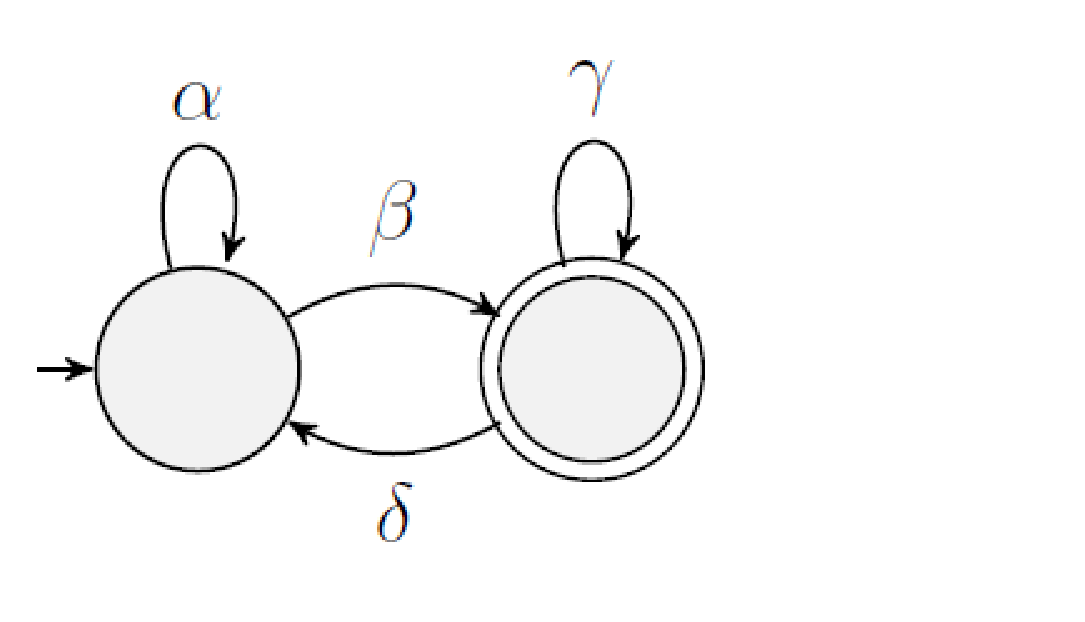
\includegraphics[width=4\linewidth]{images/1_4_4.png}
%\end{flushright} 
\end{minipage} 

Для случая, когда завершающее состояние -- это начальная вершина, регулярное выражение будет $(\gamma + \delta \alpha^* \beta)^*$.

\textit{Переход:}
\Note{Есть нестартовая и незавершающая вершина!}

1) Удаляем кратные ребра:
\begin{minipage}[r]{0.2\linewidth} 
%\begin{flushright}
    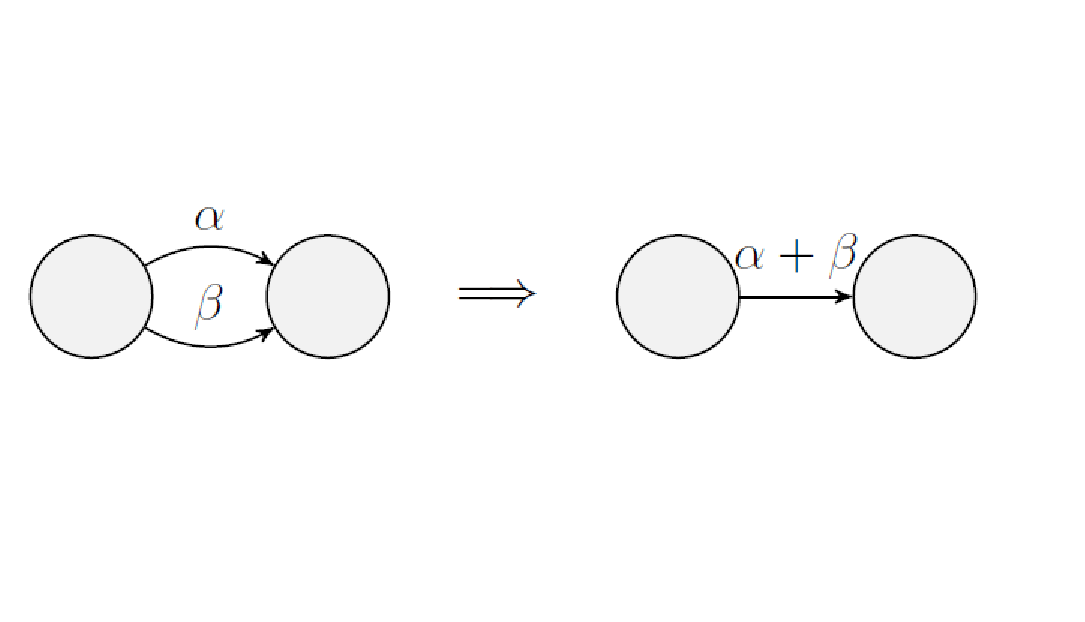
\includegraphics[width=2.5\linewidth]{images/1_4_5.png}
%\end{flushright} 
\end{minipage} 

Кратные ребра означают, что мы можем выбрать, какой символ будем использовать. Именно этот смысл и несет в себе операция <<$+$>>.

2) Добавляем циклы на себя:
\begin{minipage}[r]{0.1\linewidth} 
%\begin{flushright}
    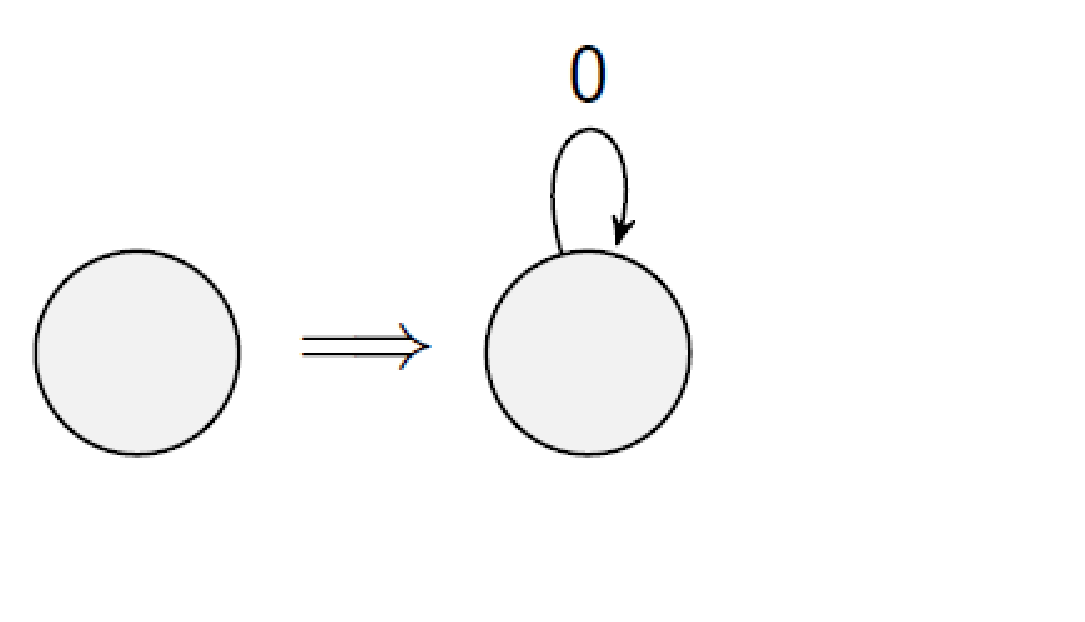
\includegraphics[width=3.5\linewidth]{images/1_4_6.png}
%\end{flushright} 
\end{minipage} 

3) Удаляем нестартовое и незавершающее состояние:

\begin{minipage}[r]{0.1\linewidth} 
%\begin{flushright}
    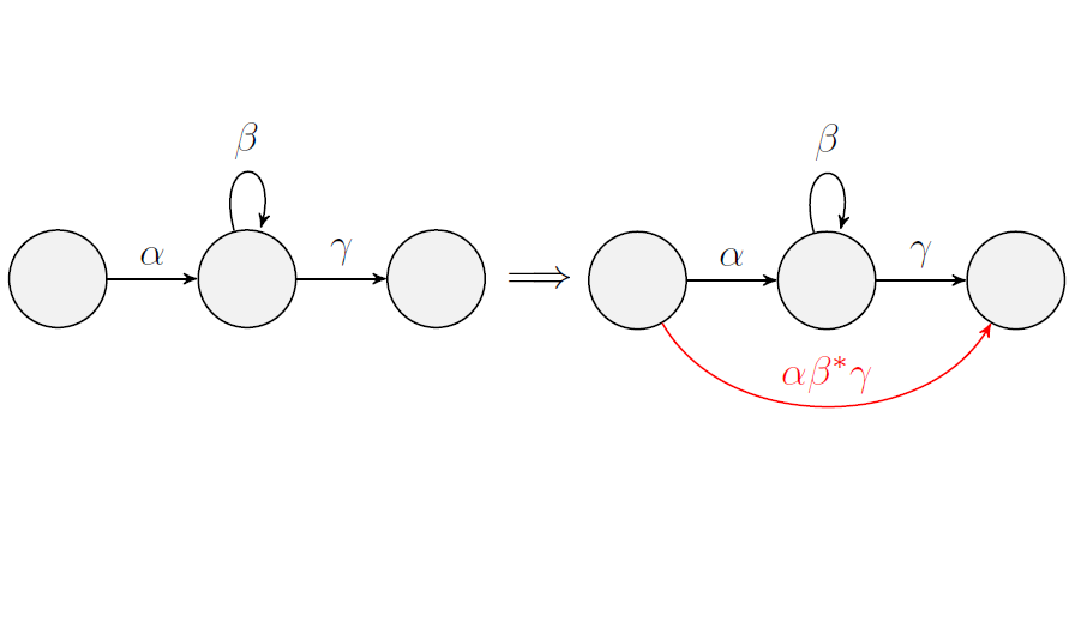
\includegraphics[width=5.5\linewidth]{images/1_4_7.png}
%\end{flushright} 
\end{minipage} 
\newline Теперь у нас на одно сотояние стало меньше, т.е. мы можем воспользоваться утверждением индукции.
\EndProof